The inference part contains in four methods.

\begin{Code}
---------------------------------- python ----------------------------------
>>> romc.sample(n2)
----------------------------------------------------------------------------
\end{Code}

\noindent
This is the basic inference utility of the ROMC implementation; we
draw $n_2$ samples for each bounding box region. This gives a total of
$k \times n_2$, where $k < n_1$ is the number of the optimal points
remained after filtering\footnote{From the $n_1$ optimisation
  problems, only the ones with $g_i(\thetab_*) < \epsilon$ are
  maintained for building a bounding box}. The samples are drawn from
a uniform distribution $q_i$ defined over the corresponding bounding
box and the weight $w_i$ is computed as in
equation~\eqref{eq:sampling}.

\begin{Code}
---------------------------------- python ----------------------------------
>>> romc.compute_expectation(h) # E[h(x)|theta]
>>> romc.eval_unorm_posterior(theta, eps_cutoff=False) # unnorm p(theta)
>>> romc.eval_posterior(theta, eps_cutoff=False) # normalised p(theta)
----------------------------------------------------------------------------
\end{Code}

\noindent
This function computes the expectation
$E_{p(\thetab|\data)}[h(\thetab)]$ using
expression~\eqref{eq:expectation}. The argument \code{h} can be any
python \code{Callable}. \code{eval_unnorm_posterior} computes the
unnormalised posterior approximation using
expression~\eqref{eq:approx_posterior}. \code{eval_posterior}
evaluates the normalised posterior estimating the partition function
$Z = \int p_{d,\epsilon}(\thetab|\data)d\thetab$; with Riemann's
integral approximation. The approximation is computationally feasible
only in low-dimensional parametric spaces.

\subsubsection*{Example - Sampling and compute expectation}

In the following code snippet, we perform weighted sampling from the
ROMC approximate posterior. Afterwards, we used some of ELFI's
built-in tools to get a summary of the obtained samples. In figure
\ref{fig:example_sampling}, we observe the histogram of the weighted
samples and the acceptance region of the first deterministic function
(as before) alongside the samples obtained from it. Finally, in the
code snippet, we demonstrate how to use the \code{compute_expectation}
function; in the current example, we define \code{h} to compute
firstly the empirical mean and afterwards the empirical variance. In
both cases, the empirical result is close to the ground truth
$\mu = 0$ and $\sigma^2 = 1$. The
\code{romc.eval_unnorm_posterior(theta)} evaluates the posterior at
point $\theta$ using expression \eqref{eq:aprox_posterior}. The
\code{romc.eval_posterior(theta)} approximates the partition function
$Z = \int_{\thetab} p_{d,\epsilon}(\thetab|\data) d\thetab$ using the
Riemann approximation as explained above. In our simple example, this
utility can provide a nice plot of the approximate posterior as
illustrated in figure~\ref{fig:approx_posterior}. We observe that the
approximation is quite close to the ground-truth posterior.

\begin{Code}
------------------------------ python snippet ------------------------------  
  # Inference part
  seed = 21
  n2 = 50
  romc.sample(n2=n2, seed=seed)

  # visualize region, adding the samples now
  romc.visualize_region(i=1)

  # Visualise marginal (built-in ELFI tool)
  romc.result.plot_marginals(weights=romc.result.weights,
                             bins=100, range=(-3,3))

  # Summarize the samples (built-in ELFI tool)
  romc.result.summary()
  # Number of samples: 19300
  # Sample means: theta: -0.0132

  # compute expectation
  exp_val = romc.compute_expectation(h=lambda x: np.squeeze(x))
  print("Expected value   : %.3f" % exp_val)
  # Expected value   : -0.013

  exp_var = romc.compute_expectation(h=lambda x: np.squeeze(x)**2)
  print("Expected variance: %.3f" % exp_var)
  # Expected variance: 1.116

  # eval unnorm posterior
  romc.eval_unnorm_posterior(theta=0)

  # check eval posterior
  romc.eval_posterior(theta=0)
----------------------------------------------------------------------------
\end{Code}

% \begin{figure}[h]
%     \begin{center}
%       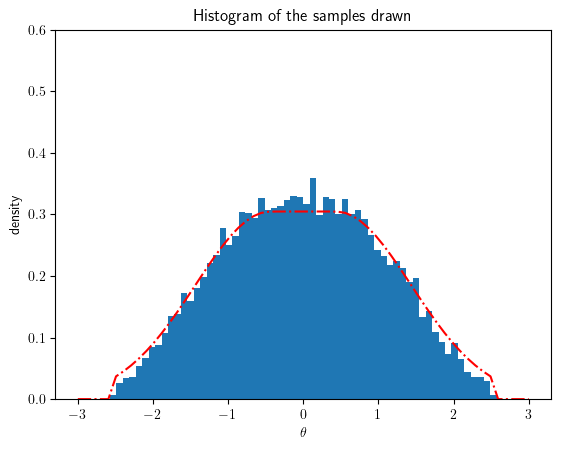
\includegraphics[width=0.48\textwidth]{./latex_files/images/chapter3/example_marginal.png}
%     \end{center}
%   \caption[Histogram of the obtained samples at the 1D example.]{(a) Left: Histogram of the obtained samples. (b) Right: Acceptance region around $\theta_1^*$ with the obtained samples plotted inside.}
%   \label{fig:example_sampling}
% \end{figure}

% \begin{figure}[h]
%     \begin{center}
%       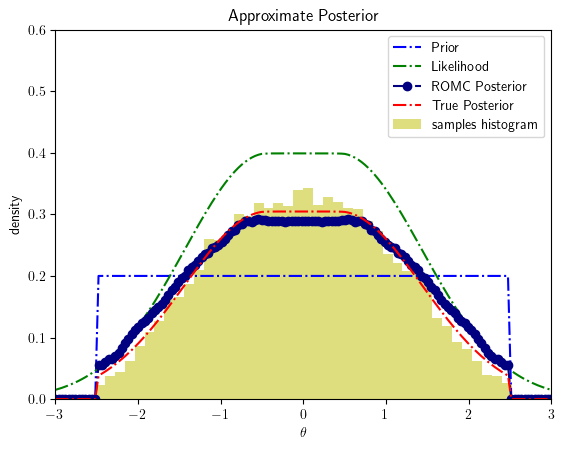
\includegraphics[width=0.6\textwidth]{./latex_files/images/chapter3/example_posterior.png}
%     \end{center}
%   \caption[Approximate posterior evaluation, at the 1D example.]{Approximate posterior evaluation.}
%   \label{fig:approx_posterior}
% \end{figure}
